\documentclass[a4paper, 11pt]{jsarticle}
\usepackage[dvipdfmx]{graphicx}
\begin{document}

\begin{titlepage}
	\begin{center}
		{\Large カレー技術特論}

		\vspace{60truept}

		{\Huge ハウス食品製カレールウ『こくまろ 中辛』を用いたカレーライスの製作\\(レポートテンプレ)}

		\vspace{180truept}

		{\Large 学籍番号: 1701999}

		\vspace{20truept}

		{\Large アイドル活動コース 1年}

		\vspace{20truept}

		{\Large 氏名: 湊みお}

		\vspace{60truept}

		{\Large 提出日: 2012年10月8日}

	\end{center}
\end{titlepage}

\section{はじめに}

カレーライスは,多種類の香辛料を用いたインド料理『カレー(curry)』を米飯にかけて食べる料理である.日本におけるカレーライスの歴史は明治時代にイギリスから伝来して以降,軍隊での食料や小中学校での給食での採用など様々な変化を遂げ,広く普及していった.\\現代では各家庭でもカレーライスが作られるようになり,様々な調理法が考案されている一方で,カレールウメーカー・ハウス食品株式会社は箱の裏に記載されている調理法での製作を推奨している.そこで,本稿では有名なカレーライスの独自調理法を挙げるとともに,箱の裏に記載されている調理法に従って製作したカレーライスの評価・性能試験を実施する.

\section{有名な独自調理法}

個人の味覚の好みにあわせて調理する際,カレールウの箱の裏に記載されている調理具材にはない様々な食材を,カレーを煮込む際などに投入することがある\cite{arrange}.ここでは,加えたい『好みの味』に合わせた食材について述べる.

\subsection{リンゴ}
リンゴをすりおろして煮込むことにより,リンゴ由来の酸味と甘さ,まろやかさが加わり,マイルドなカレーに変化する.特に,豚肉を用いたカレーに有効であることが分かっている.

\subsection{ハチミツ}
リンゴと同様,甘さとまろやかさを加える効果がある.一方で市販のハチミツにはアミラーゼ等の消化酵素が含まれており,とろみの主成分であるデンプンを分解する作用があるが,十分な加熱処理を加えて酵素の働きを抑えることで,とろみを維持したままハチミツの作用を加えることができる.

\subsection{トマト}
トマトを加えることによりさわやかさと酸味を加えることができる.生のトマトを入れる方法や,トマト缶,トマトジュースなど加工品を入れるものなど様々な手法が考案されている.また,トマトに含まれるアスパラギン酸やグルタミン酸などの旨味成分でコクのある味わいを加えることも可能である.

\section{提案手法}
ここみてください...↓\\
\texttt{https://housefoods-group.com/activity/e-mag/magazine/04.html}

\begin{figure}[htb]
	\begin{center}
		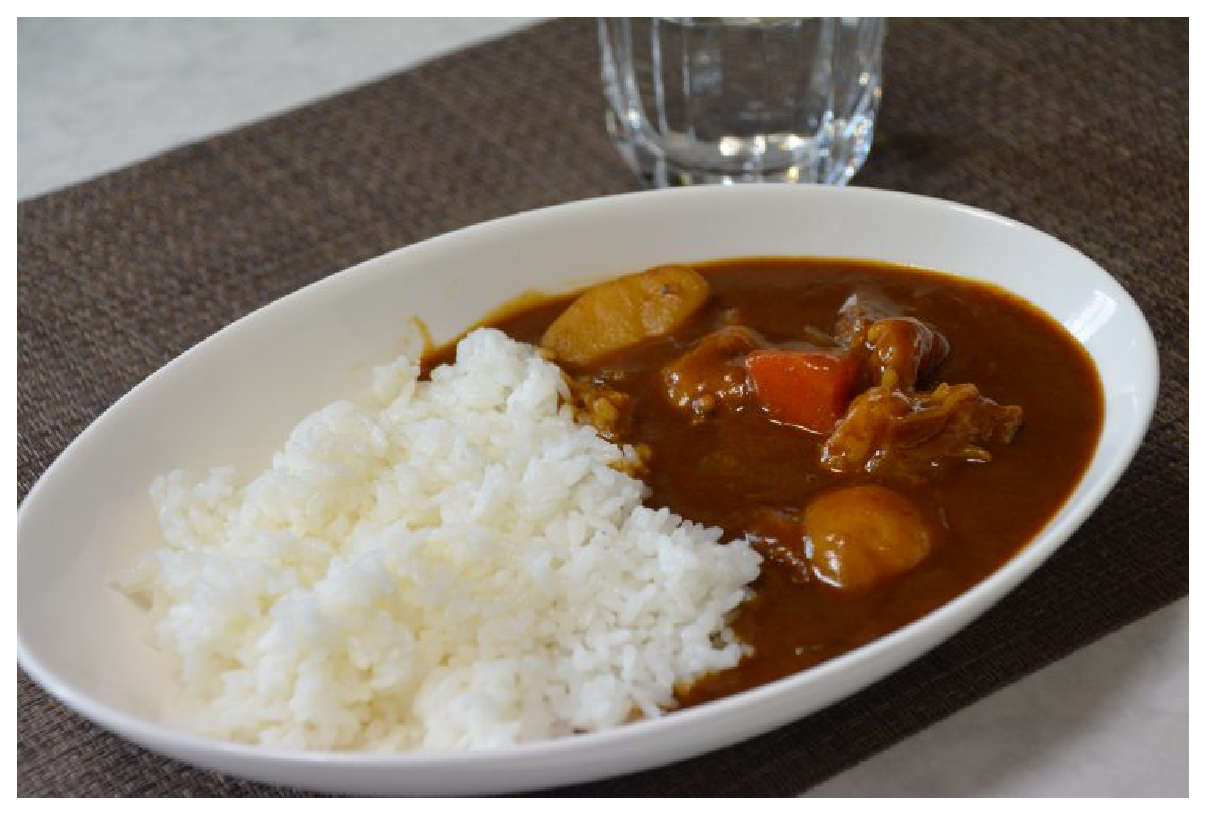
\includegraphics[clip,width = 5.0cm]{curry.eps}
	\end{center}
	\caption{カレーライスのフリー画像}  \label{curryfig}
\end{figure}

\begin{table}[htb]
	\caption{カレーの材料(8皿分)}
	\centering
	\begin{tabular}{lcr}
		\hline
		食材 & 目安 & 分量 \\
		\hline\hline
		こくまろカレー(中辛) & 1箱 & 140g\\
		肉 & - & 300g\\
		玉ネギ & 中2個 & 400g \\
		ジャガイモ & 中2個 & 300g \\
		ニンジン & 中1本 & 200g \\
		サラダ油 & 大さじ2 & 30mL \\
		水 & - & 1000mL \\
		\hline
	\end{tabular}
\end{table}

\section{考察}

実験の結果,おいしいカレーができた.シンプルだけどとてもおいしかったです.

\section{まとめ}

おいしいカレー作った.

\section{参考文献}
\begin{thebibliography}{9}
	\bibitem{arrange}
	{ハウス食品株式会社},``カレーの隠し味 | こだわりカレー術''ハウス食品グループ株式会社 , https://housefoods.jp/data/curryhouse/cook/lesson/secret.html, accessed July. 26, 2021.
\end{thebibliography}


\end{document}